
\medskip

\begin{enumerate}
\item $f'(x) = \left(4x - 1\right) \times \e^x + 4 \times \e^x = \e^x \left(4x - 1 + 4\right) = \e^x (4x + 3).$

\item Résolution de $f'(x) = 0$, soit $\e^x (4x + 3) = 0$.

$\e^x > 0$, donc : $\quad 4x + 3 = 0 \quad \Longrightarrow \quad x = -\dfrac{3}{4}$.

Valeur en $x = -\dfrac{3}{4}$ :
\[f\left(-\dfrac{3}{4}\right) = \left(4 \times \left(-\dfrac{3}{4}\right) - 1\right)\e^{-\frac{3}{4}} = (-3 - 1)\e^{-\frac{3}{4}} = -4\e^{-\frac{3}{4}}.\]

\begin{center}
\begin{tikzpicture}
\tkzTabInit[lgt=2.5, espcl=3]{$x$ / 1, {$\e^x$} / 1, {$4x + 3$} / 1, {Signe de $f'(x)$} / 1, {Variations de $f$} / 2}{${-1}$, ${-\frac{3}{4}}$, ${+\infty}$}
\tkzTabLine{,+,d,+,}
\tkzTabLine{,-,0,+,}
\tkzTabLine{,-,0,+,}
\tkzTabVar{+/{$$},-/{$-4\e^{-\frac34}$},+/{$$}}{/}
\end{tikzpicture}
\end{center}

\end{enumerate}

\bigskip

